%%%%%%%%%%%%%%%%%%%%%%%%%%%%%%%%%%%%%%%%%
% Wenneker Assignment
% LaTeX Template

% Version 2.0 (12/1/2019)
%
% This template originates from:
% http://www.LaTeXTemplates.com
%
% Authors:
% Vel (vel@LaTeXTemplates.com)
% Frits Wenneker
%
% License:
% CC BY-NC-SA 3.0 (http://creativecommons.org/licenses/by-nc-sa/3.0/)
% 
%%%%%%%%%%%%%%%%%%%%%%%%%%%%%%%%%%%%%%%%%

%----------------------------------------------------------------------------------------
%	PACKAGES AND OTHER DOCUMENT CONFIGURATIONS
%----------------------------------------------------------------------------------------

\documentclass[12pt]{scrartcl} % Font size

%%%%%%%%%%%%%%%%%%%%%%%%%%%%%%%%%%%%%%%%%
% Wenneker Assignment
% Structure Specification File
% Version 2.0 (12/1/2019)
%
% This template originates from:
% http://www.LaTeXTemplates.com
%<
% Authors:
% Vel (vel@LaTeXTemplates.com)
% Frits Wenneker
%
% License:
% CC BY-NC-SA 3.0 (http://creativecommons.org/licenses/by-nc-sa/3.0/)
% 
%%%%%%%%%%%%%%%%%%%%%%%%%%%%%%%%%%%%%%%%%

%----------------------------------------------------------------------------------------
%	PACKAGES AND OTHER DOCUMENT CONFIGURATIONS
%----------------------------------------------------------------------------------------

\usepackage{amsmath, amsfonts, amsthm} % Math packages

\usepackage{listings} % Code listings, with syntax highlighting

\usepackage[francais]{babel} % English language hyphenation
\usepackage[final]{pdfpages}

\usepackage{graphicx} % Required for inserting images
\graphicspath{{Figures/}{./}} % Specifies where to look for included images (trailing slash required)

\usepackage{booktabs} % Required for better horizontal rules in tables
\usepackage{adjustbox}
\numberwithin{equation}{section} % Number equations within sections (i.e. 1.1, 1.2, 2.1, 2.2 instead of 1, 2, 3, 4)
\numberwithin{figure}{section} % Number figures within sections (i.e. 1.1, 1.2, 2.1, 2.2 instead of 1, 2, 3, 4)
\numberwithin{table}{section} % Number tables within sections (i.e. 1.1, 1.2, 2.1, 2.2 instead of 1, 2, 3, 4)

\setlength\parindent{0pt} % Removes all indentation from paragraphs

\usepackage{enumitem} % Required for list customisation
\setlist{noitemsep} % No spacing between list items

%----------------------------------------------------------------------------------------
%	DOCUMENT MARGINS
%----------------------------------------------------------------------------------------

\usepackage{geometry} % Required for adjusting page dimensions and margins

\geometry{
	paper=a4paper, % Paper size, change to letterpaper for US letter size
	top=2.5cm, % Top margin
	bottom=3cm, % Bottom margin
	left=3cm, % Left margin
	right=3cm, % Right margin
	headheight=0.75cm, % Header height
	footskip=1.5cm, % Space from the bottom margin to the baseline of the footer
	headsep=0.75cm, % Space from the top margin to the baseline of the header
	%showframe, % Uncomment to show how the type block is set on the page
}

%----------------------------------------------------------------------------------------
%	FONTS
%----------------------------------------------------------------------------------------

\usepackage[utf8]{inputenc} % Required for inputting international characters
\usepackage[T1]{fontenc} % Use 8-bit encoding

\usepackage{fourier} % Use the Adobe Utopia font for the document

%----------------------------------------------------------------------------------------
%	SECTION TITLES
%----------------------------------------------------------------------------------------

\usepackage{sectsty} % Allows customising section commands

\sectionfont{\vspace{6pt}\centering\normalfont\scshape} % \section{} styling
\subsectionfont{\normalfont\bfseries} % \subsection{} styling
\subsubsectionfont{\normalfont\itshape} % \subsubsection{} styling
\paragraphfont{\normalfont\scshape} % \paragraph{} styling

%----------------------------------------------------------------------------------------
%	HEADERS AND FOOTERS
%----------------------------------------------------------------------------------------

\usepackage{scrlayer-scrpage} % Required for customising headers and footers

\ohead*{} % Right header
\ihead*{} % Left header
\chead*{} % Centre header

\ofoot*{} % Right footer
\ifoot*{} % Left footer
\cfoot*{\pagemark} % Centre footer
 % Include the file specifying the document structure and custom commands
\usepackage{hyperref}
 
\urlstyle{same}
%----------------------------------------------------------------------------------------
%	TITLE SECTION
%----------------------------------------------------------------------------------------

\title{	
	\normalfont\normalsize
	\textsc{CNAM}\\ % Your university, school and/or department name(s)
	\vspace{25pt} % Whitespace
	\rule{\linewidth}{0.5pt}\\ % Thin top horizontal rule
	\vspace{20pt} % Whitespace
	{\huge Projet RCP208 : Compte Rendu TD}\\ % The assignment title
	\vspace{12pt} % Whitespace
	\rule{\linewidth}{2pt}\\ % Thick bottom horizontal rule
	\vspace{12pt} % Whitespace
}

\author{\LARGE Jérôme Petit} % Your name

\date{\normalsize\today} % Today's date (\today) or a custom date

\begin{document}

\maketitle % Print the title


\section{TD K-means}
\subsection{CR : variable uniforme}
Je génère 500 variables uniformes auquel j'associe 5 étiquettes (1,2,3,4,5), ci dessous un exemple de données générées~:
\newline
\begin{figure}[!h]
 \centering 
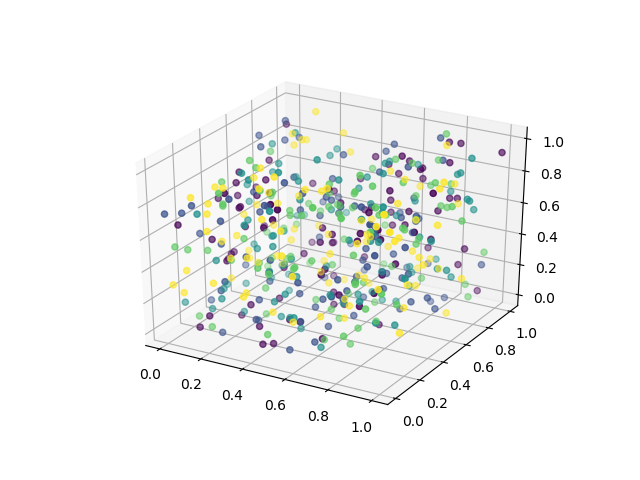
\includegraphics[scale=.5]{uniform.png}
\end{figure}
\newline
En appliquant une classification par K-means avec les paramètres : n\_init=1, nb\_clusters =5 et initialisation : k-means++, on obtient les données suivantes : 
\newline
\begin{figure}[!h]
 \centering 
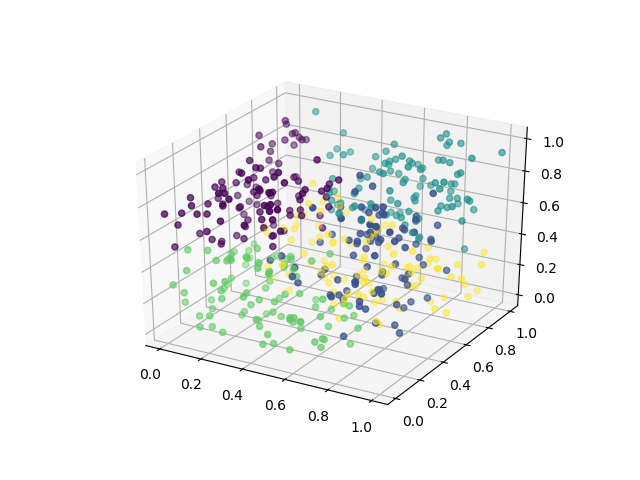
\includegraphics[scale=.5]{uniformKmeans.png}
\end{figure}
\newline
Afin de déterminer la qualité de la classification j'ai utilisé la métrique de Rand ajusté et de Jacquard. Pour l'échantillon précédent je trouve une valeur de 0.0059947710270688665 pour Rand ajusté et 0.176 pour Jacquard. Les valeurs obtenues sont très faibles par rapport à des données normales et séparés. Cette valeur faible provient du faite qu'il n'y a pas de cluster apparent, il est donc impossible d'avoir une séparation cohérente des données. 

Les résultats obtenues sont stables, en effet en faisant 10 classifications, on obtient les résultats suivant~: indice de Rand ajusté : moyenne 0.0048179719511162265 et écart type :0.0025297897570419775

Si l'on utilise la même approche pour la génération de variables normales (on génére les variables puis on les sépare afin d'avoir des clusters) alors on a les données suivantes :
\newline
\begin{figure}[!h]
 \centering 
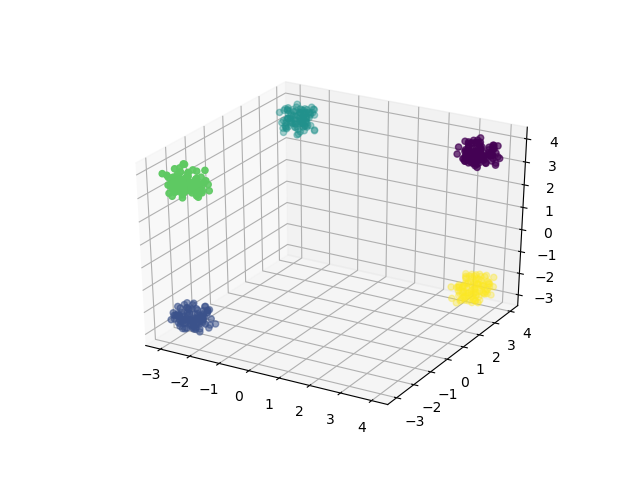
\includegraphics[scale=.3]{unifor_lag.png}
\end{figure}
\newline
En appliquant une classification par K-means avec les paramètres : n\_init=1, nb\_clusters =5 et initialisation : k-means++, on obtient les données suivantes : 
\newline
\begin{figure}[!h]
 \centering 
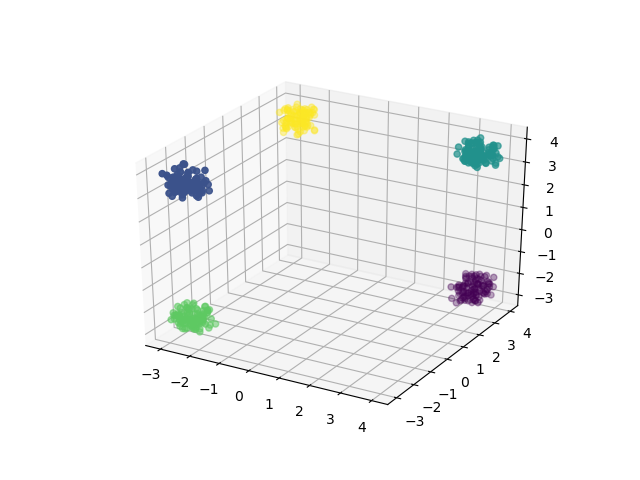
\includegraphics[scale=.3]{uniform_lagKmeans.png}
\end{figure}
\newline
Dans ce cas on obtient des résultats légèrement meilleur à ceux obtenues par variables normales. Ce résultat est cohérent avec la méthode K-means. Cette méthode détecte les clusters et n'est pas sensible à la distribution des variables. Les résultats sont donc légèrement meilleur car on a  dans le cas uniforme les clusters sont plus disjoint que dans le cas normale. Pour les variables uniformes après avoir fait 10 classification K-means (avec initialisation k-means++, nb\_cluster=5 et n\_init=1) j'obtiens un indice de rand ajusté en moyenne de 1.0 et d'écart type 0.0.
\subsection{CR : Texture}
En appliquant le l'approche K-means avec 11 cluster, une initialisation K-means++ et n\_init=1, on obtient un score de Rand ajusté 0.46479949030200746. Ce qui est faible. Cela vient du fait que l'on utilise l'algorithme K-means sur des données ayant 40 variables. Afin de réduire ce nombre de variable et de faire apparaitre les axes contenant l'information nécessaire on utilise une approche discriminante. En utilisant 10 axes, on obtient les ratio de variances suivant : axe 1 : 45.86\%, axe 2 : 24.24\%, axe 3 : 9.65\% , axe 4 : 6.94\%, axe 5 :  5.54\% , axe 6 : 2.42\%, axe 7 :
 2.26\%, axe 8 : 1.56\% axe 9 : 0.84\% et l'axe 10: 0.68\%. CE qui signifie que les 5 premiers axes représente 90\% de la variance. Grace à l'analyse factoriel on s'est ramené à 10 variables. En appliquant alors le même algorithme K-means on a cette fois ci un score de Rand ajusté de 0.9956363636363637. Afin de déterminé quel est la projection optimal j'ai réalisé la méthode classification pour des nombres de composants allant de 1 à 20. Le score de rand ajusté obtenu par le K-means est le suivant : 
\newline
\begin{figure}[!h]
 \centering 
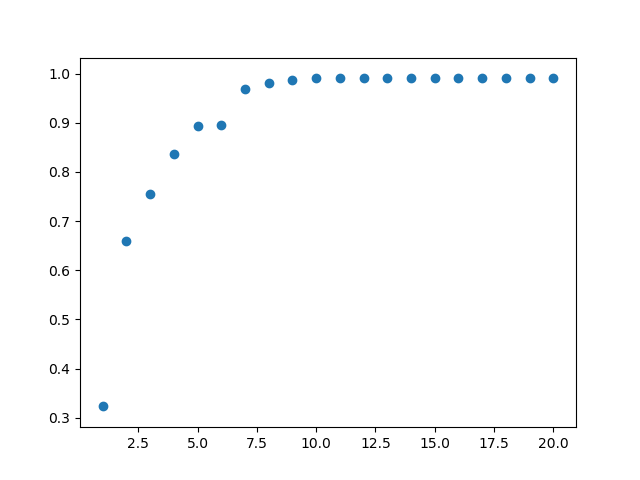
\includegraphics[scale=.3]{AFD_K_means.png}
\end{figure}
\newline 
Ainsi une AFD à 8 composants va donner un résultat similaire à une AFD à 20 composants. Ci dessous est le jeu de données initial projeté sur les 3 premiers axes~: 
\newline
\begin{figure}[!h]
 \centering 
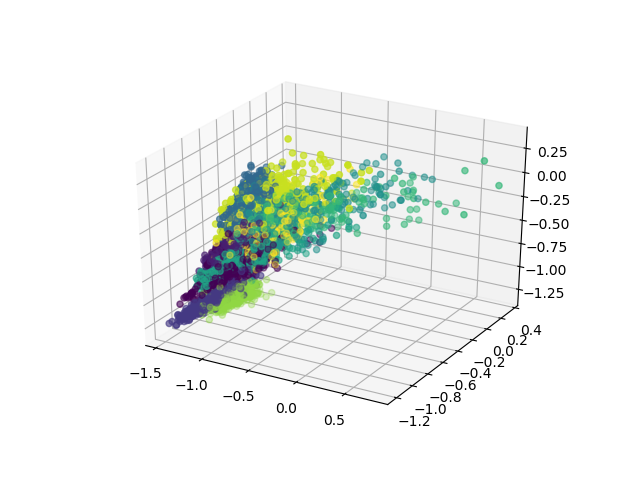
\includegraphics[scale=.5]{init.png}
\end{figure}
\newline 

On ne voit pas apparaitre clairement de cluster. A l'aide de l'AFD on va pouvoir changer le nombre de variables tout en préservant la dispersion en utilisant 8 axes~:
\newline
\begin{figure}[!h]
 \centering 
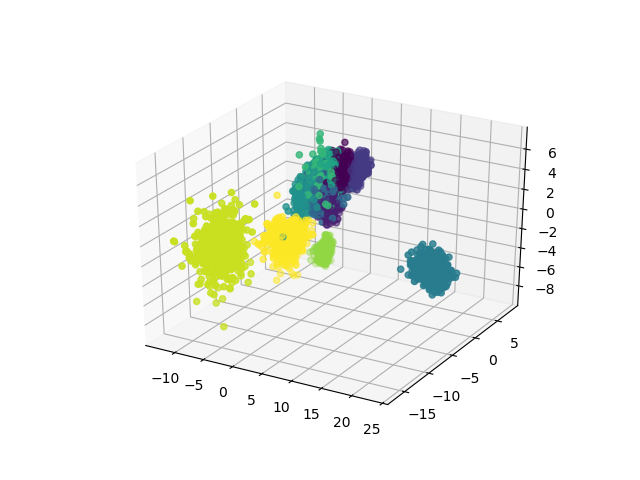
\includegraphics[scale=.5]{AFD8.png}
\end{figure}
\newline 

Les clusters apparaissent plus clairement en utilisant une classification K-means avec 11 clusters et une initialisation K-means++, on obtient la classification suivante~:
\newline
\begin{figure}[!h]
 \centering 
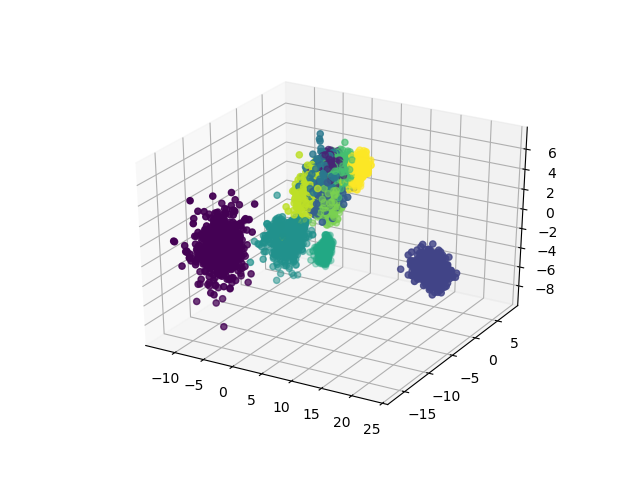
\includegraphics[scale=.5]{kmeans_AFD8.png}
\end{figure}
\newline 
\section{Classification spectrale}
\subsection{Variable uniforme}
Comme pour le TD K-means j'ai généré des données suivant la loi uniform  [0,1]. Ci dessous se trouve les données générées : 
\newline
\begin{figure}[!h]
 \centering 
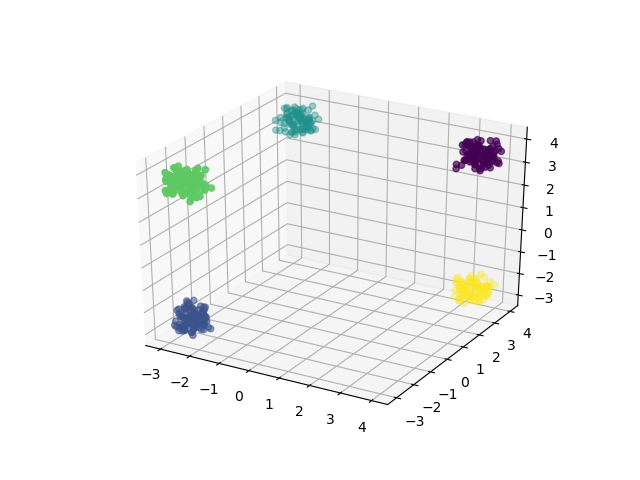
\includegraphics[scale=.5]{unifSpectrale.png}
\end{figure}
\newline 
En appliquant l'analyse spectrale sur les données en utilisant la méthodes de proches voisins pour la création de la matrice de similiarité on remarque une instabilité des résultats. Ci dessous se trouve les valeurs de l'indice de rand ajusté en fonction du nombre n\_neigboorhood choisi (entre 1 et 20) : 
\newline
\begin{figure}[!h]
 \centering 
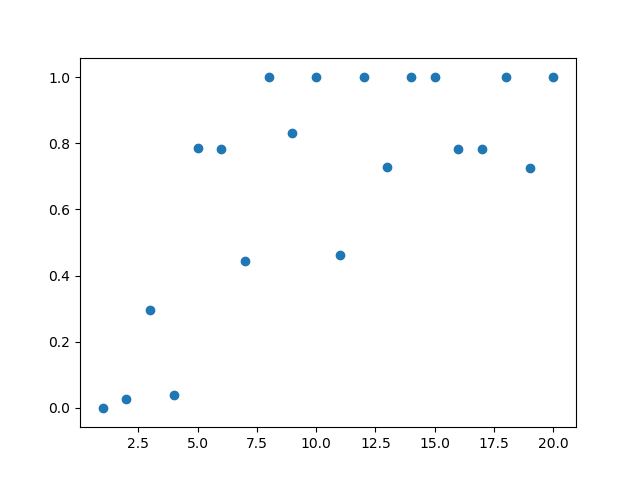
\includegraphics[scale=.5]{spectralUnifNN.png}
\end{figure}
\newline 
Par contre comme dans le cas normal on observe une tres bonne classification par le noyau rbf pour des valeurs de $\gamma\leq 8$ (indice de rand ajusté vaut 1). La classification est moins stable pour des valeurs de $\gamma >8$. 
\newline
\begin{figure}[!h]
 \centering 
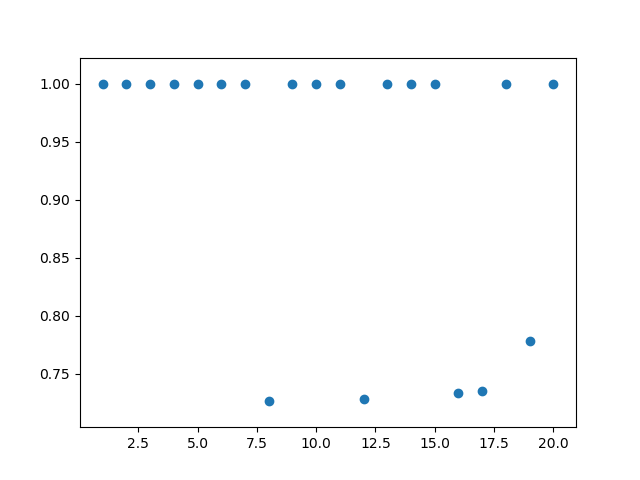
\includegraphics[scale=.5]{spectralUnifRBF.png}
\end{figure}
\newline 
L'approche par K-means est beaucoup plus stable que l'analyse spectrale avec l'approche par K-means on a un indice de rand ajusté de 1.0 avec une initialisation k-means++. L'approche k-means est de meilleur qualité avec une initialisation k-means++ car les cluster sont disjoints ce qui rend adapté pour cette méthode. De plus l'analyse spectrale donne de moins bon résultats pour gamma > 8 car il y a trop de composantes connexes. Pour des valeurs inférieur à 8 les résultats sont similaire à l'approche k-means.
\subsection{données : Texture}
Sans appliquer l'AFD afin de réduire la dimension, la classification spectrale avec la méthode des proches voisins et n\_neighborhood=9$\approx$ log(5500)+1 donne un indice de rand ajusté de 0.6007141289011186. Afin d'améliorer ce résultat, j'utilise une AFD qui va réduire la nombre de variables afin de les regrouper de la plus explicative à la moins. Ce critère est donné par la variance. Comme pour l'étude K-means, nous observons que 8 composantes donne un résultat similaire à 20 composantes. En appliquant une méthode spectrale après avoir appliqué une AFD à 8 composantes. on obtient la classification suivante (projection sur les 3 premières composantes)
\newline
\begin{figure}[!h]
 \centering 
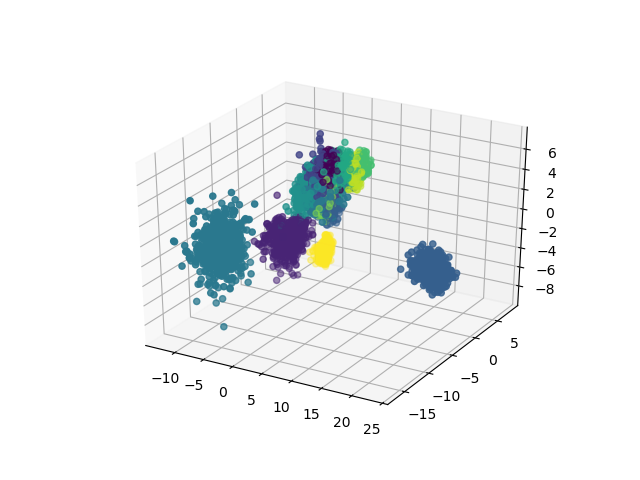
\includegraphics[scale=.5]{spectraleAFD.png}
\end{figure}
\newline 
Avec 8 composantes pour l'AFD et la méthode spectrale par proche voisin (n\_neighborhood = 9) on obtient un indice de rand ajusté de 0.8146208480795527. Contrairement à la méthode K-means la stabilité des résultats est moindre, cela vient du nombre de composante connexe en jeu. Ci dessous la valeur de l'indice de rand ajusté en fonction du nombre de composant dans l'AFD (la méthode spectrale utilisée est proche voisin avec 9 voisins)
\newline
\begin{figure}[!h]
 \centering 
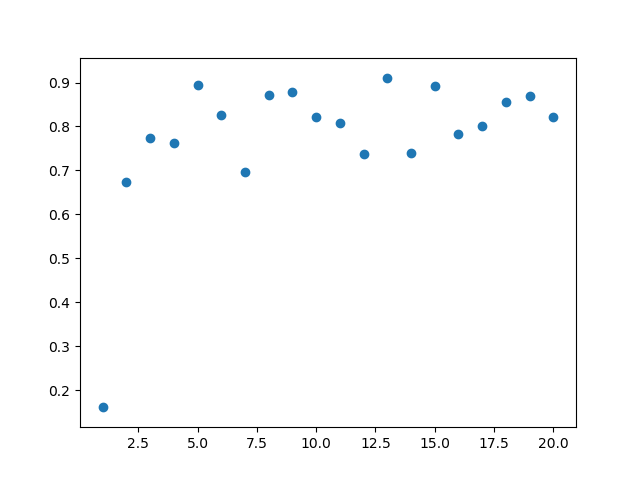
\includegraphics[scale=.3]{metricsAFDNN.png}
\end{figure}
\newline 
\section{TD : mélange de densité}
En utilisant 100 données et 2 composantes la densité obtenue est proche de la vraie densité, la valeur de la log vraisemblance est de -2.0139415707841097~:
\newline
\begin{figure}[!h]
 \centering 
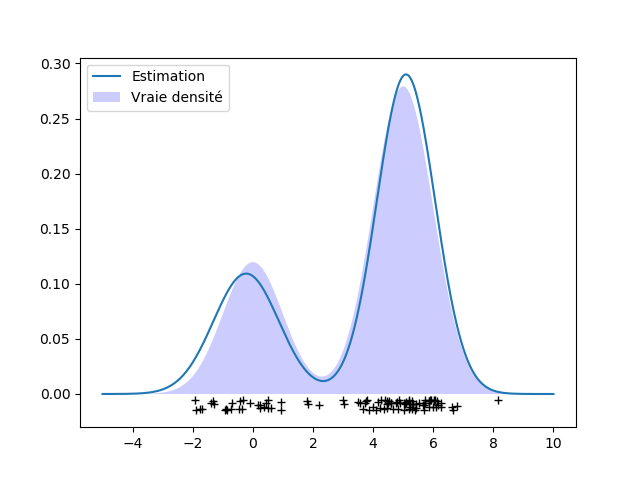
\includegraphics[scale=.3]{densite100.png}
\end{figure}
\newline 
En augmentant le nombre d'échantillon : N=10000, on obtient une log vraisemblance de : -2.011940707075323. La densité obtenue correspond exactement à la vrai densité : 
\newline
\begin{figure}[!h]
 \centering 
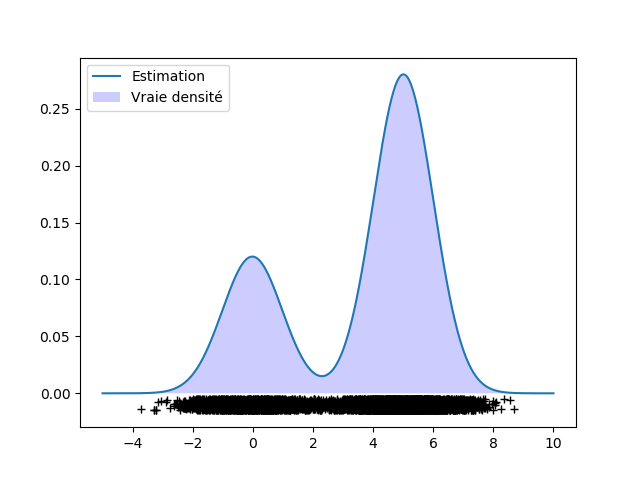
\includegraphics[scale=.3]{densite10000.png}
\end{figure}
\newline 
Étant donné que la qualité de l'estimation pour N=10000 est sensiblement meilleur que pour N=100, j'ai étudié l'évolution de la log vraisemblance en fonction du nombre de composante pour N=100. Ci dessous le graphe de la log vraisemblance en fonction du nombre de composantes utilisées dans l'estimation (entre 1 et 20) : 
\newline
\begin{figure}[!h]
 \centering 
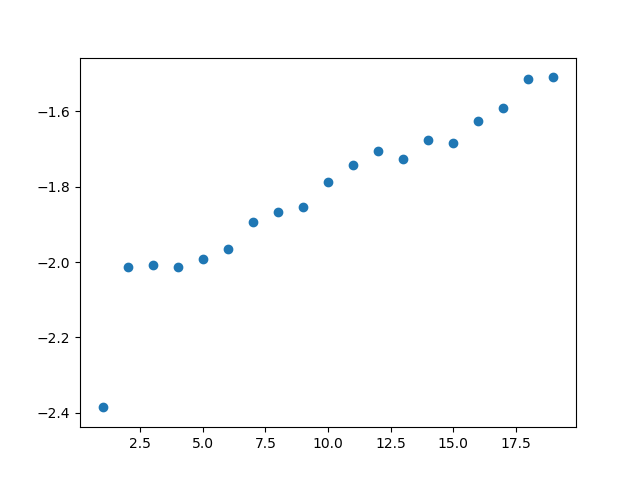
\includegraphics[scale=.3]{log100.png}
\end{figure}
\newline 
On observe que plus le nombre de composantes plus la log vraisemblance augmente. MAis l'augmentation du nombre de composantes nécessite plus de données en effet pour N=100 on a~:
\newline
\begin{figure}[!h]
 \centering 
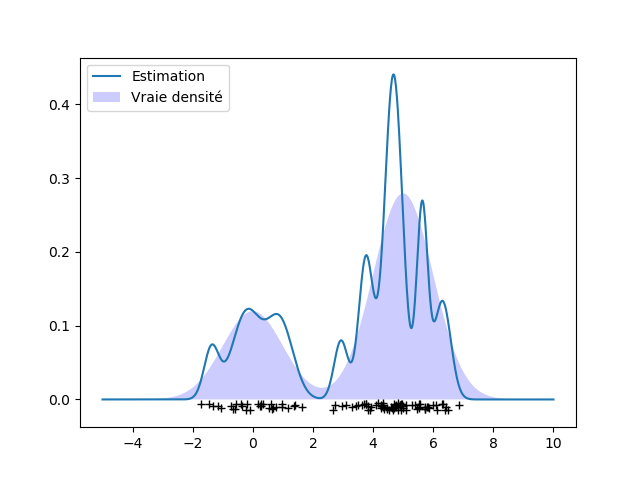
\includegraphics[scale=.3]{densite8cpt.png}
\end{figure}
\newline 
En utilisant 10000 données l'approximation est meilleure qualité mais l'approximation reste de moins bonne qualité que celle obtenue avec 2 composantes~:
\newline
\begin{figure}[!h]
 \centering 
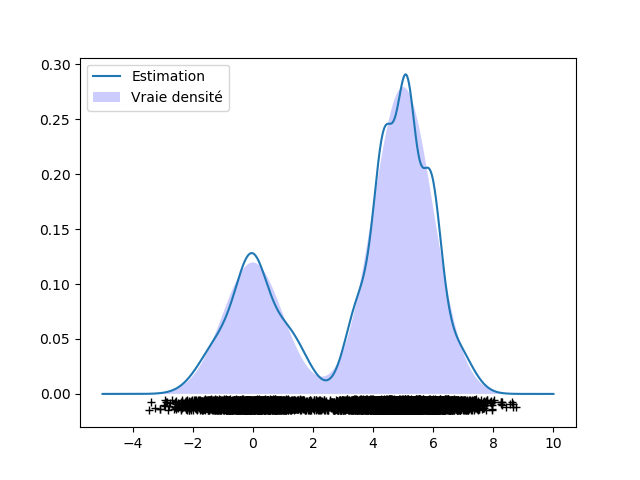
\includegraphics[scale=.3]{densite8cpt10000.png}
\end{figure}
\newline  
\subsection{critere AIC}
En utilisant diag au lieu de full dans l'estimation, on obtient la même classification les minimum des critères AIC et BIC sont obtenues pour 3 composantes. Dans le cas diag le minimum AIC est plus faible que dans le cas full~:
\newline
\begin{figure}[!h]
 \centering 
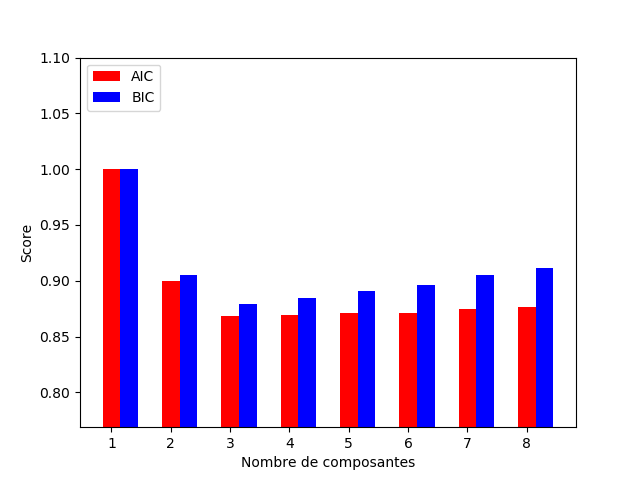
\includegraphics[scale=.4]{barAIC.png}
\end{figure}
\newline  
\end{document}